\documentclass[a4paper,8pt,french,fleqn]{article}
%Packages:

\usepackage{graphicx}

%Langages:
\usepackage[french]{babel}
\usepackage{lmodern}
\usepackage[T1]{fontenc}
\usepackage[utf8]{inputenc}

%Mise en page
\usepackage[top=2cm, right=2cm, bottom=2cm, left=2cm]{geometry}
\usepackage{fancyhdr}
\usepackage{enumerate}
\usepackage{color}

%Titre et auteurs
\title{\textbf{Compilation}\\\textit{Rapport}}

\author{PHILIPPI Alexande \& MAUPEU Xavier \& FIOT Arthur \& DEVOIR Loïc}

\date{\today}

\begin{document}
\maketitle

\clearpage

\section*{Equipe}

L'équipe est constituée de MAUPEU Xavier, FIOT Arthur, DEVOIR Loïc et PHILIPPI Alexandre. Tous les quatre nous sommes du groupe 4 de travaux dirigés, avec comme encadrant Mr. SERGENT Marc.


\section{Implémentation}

Notre implémentation est basée sur le langage C. Pour cela nous nous sommes penchés sur différents points.

\subsection{Types supportés}

Les types implémentés sont \textit{float} et \textit{int}, tableaux statiques et dynamiques de \textit{float} et \textit{int}. Le compilateur gère les variables et tableaux globaux.

\subsection{Fonctions}

On peut déclarer les fonctions externes grâce à des prototypes. Les paramètres peuvent etre des \textit{int}, des \textit{float} et des tableaux dynamiques.
Les fonctions \textit{printint(int)} et \textit{printfloat(float)} sont prédéfinies et peuvent être utilisées par l'utilisateur.

\subsection{Expressions}

Le compilateur gère les opérations courantes telles que "+", "-" , "*", "!","<",">","<=",">=","!=" et "==" entre deux variables de même type.\\

\subsection{Instructions}

Le compilateur gère les affectations, les boucles \textit{for} et \textit{while}, les blocs d'instructions et le \textit{if} (qui peut avoir ou non un \textit{else}).


\section{Codage du compilateur}
Le compilateur a été réalisé en C++ 11 afin de pouvoir utiliser une approche objet des instructions (fig. \ref{archi}). Les classes \textit{std::string} et \textit{std::ostringstream} nous ont aussi été très utiles.

\begin{figure}[h!]
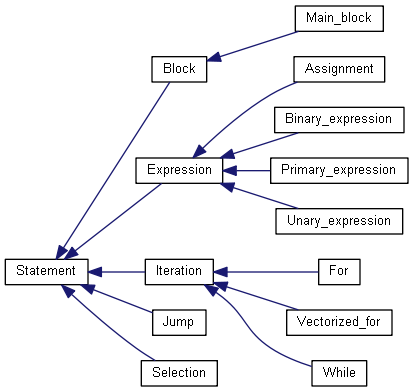
\includegraphics[scale = 0.8]{inherit_graph.png}
\caption{Graphe représentatif de l'architecture}
\label{archi}
\end{figure}

\subsection{Gestion des erreurs}

La syntaxe du code lu est vérifiée grâce à la grammaire, mais cela ne suffit pas: par exemple, l'affectation d'un \textit{float} dans une variable de type \textit{int} provoque un comportement indéterminé à l'exécution. Pour cela nous avons choisi d'utiliser le système de gestion d'exceptions du c++. Le compilateur gère ainsi 38 types d'erreurs différentes parmi lesquelles : 
\begin{itemize}
\item les types interdits (comme le type void),
\item variables ou fonctions non déclarées,
\item affectation d'une variable d'un mauvais type,
\item des types non correspondants pour les opérateurs binaires,
\item des types non correspondants pour les opérateurs unaires,
\item non concordance des arguments lors de l'appel d'une fonction,
\item fonction void qui retourne une valeur,
\item fonction qui retourne un type différent du type de retour déclaré.
\end{itemize}

\subsection{Les types flottants}
Le stockage des flottants se fait sur la pile et prend à chaque fois 4 octets. Pour toutes les opérations nécessitant de manipuler des flottants comme les affectations ou les opérations binaires, on charge la valeur stockée sur la pile dans un registre de travail $\%xmm*$. Nous avons choisi de ne pas utiliser les registres AVX car deux de nos ordinateurs ne pouvaient pas les exécuter. 

\section{Boucles for vectorielles}
L'extension implémentée est la ``Boucle \textit{for} vectorielle'' via les deux pragmas : ``\#pragma omp simd'' et ``\#pragma omp simd reduction(+: id)''.

\subsection{Vectorisation à l'aide des instructions SIMD}

La boucle \textit{for} ne devra comporter que des affectations sur des flottants et sera de la forme:\\
$for (i=cst1 ; i<cst2 ;i++) \{ \\
(assignments) \\
\}\\$
avec \textit{i} une variable quelconque et $cst*$ des constantes quelconques.
Le nombre de tour de boucle, c'est à dire $cst2 - cst1$, doit être un multiple de 4.\\
Pour ce type de boucle, la variable \textit{i} est incrémentée de 4 à chaque fois. Lors du chargement ou du stockage d'une case \textit{i} d'un tableau dans un registre $\%xmm*$, on en profite pour charger ou stocker aussi la case \textit{i+1}, \textit{i+2}, \textit{i+3} car les registres font 128 bits.\\
On peut faire des opérations entre : 
\begin{itemize}
\item des tableaux et des constantes, ex : $A[i] + 5.0$,
\item des tableaux et des variables locales ou globales, ex : $A[i] + b$,
\item des tableaux et des fonctions, ex : $A[i] + sqrtf(b)$.
\end{itemize}

\subsection{Réduction d'une variable}
En utilisant la ligne ``\#pragma omp simd reduction(+: id)' avant un \textit{for}, on peut utiliser dans le corps de la boucle l'affectation : $id = id + ...;$.
Pour cela on somme les 4 éléments d'un registre $\%xmm*$, et on le stocke dans la variable \textit{id}.

\end{document}
